\rhead{引言}
\chapter{引言}
%@@@@@@@@@@@@@@@@@@@@@@@@@@@@@@@@@@@@@@@@@@@@@@
\section{研究背景及意义}
生物学研究的一个重要目标,就是理解生命细胞中各个组成部分的功能以及它们之间的联系。其中,蛋白质(protein)是具有极其重要意义的生物结构,它能帮助我们理解细胞作用的机理。分析蛋白质序列以及比较不同蛋白质之间的序列相似性,都能帮助我们充分理解蛋白质的功能及作用。

但是,近年来,蛋白质被发现其往往不是单一活动的。生物的细胞生命活动,是需要许多蛋白质在一起相互作用,才能够完成的,而并不是靠某个单一的蛋白质就能做到的。发现并理解蛋白质与蛋白质之间的相互作用(protein-protein interactions,PPIs),就成为了领域内的重要课题之一。

伴随着这一新课题,许多新的生物学实验\cite{uetz2000comprehensive,ito2001comprehensive,krogan2006global,han2004evidence,nabieva2005whole,yook2004functional}被设计了出来,这些实验的目的便是发现蛋白质之间的相互作用结构。而这些大量的实验结果,急需一个合适的数学模型来对它们进行建模,以便于学者们的与实验与分析。

因此,学者们就提出了蛋白质相互作用网络(protein-protein interaction networks)这一图论模型。在有了PPI网络这一模型后,类似于通过匹配不同基因组序列以分析基因组的方法,通过匹配两种生物间的PPI网络,也能够成为分析生物细胞体内蛋白质相互作用的一种方法。而且,PPI网络之间的匹配,不但能够利用生物蛋白质之间的序列相似性,也能够利用网络之间的拓扑结构相似性,比起之前单一比较蛋白质序列相似性的方法,要好的多。

PPI网络匹配(PPI network alignment,NA)是将两个不同物种的PPI网络进行匹配的过程。NA的目的在于找到两个PPI网络中极为相似的一些区域,这个相似,从不同的研究问题来看,可以有不同的意义,可以是生物功能的相似,也可以是拓扑结构的相似。但无论是哪种相似的定义,PPI网络匹配的好坏,具有极其重要的的作用。一个好的PPI网络匹配,能够找到两个PPI网络中十分相似的子结构,从而能够把一种生物的知识体系,完全借鉴在另一种未知PPI网络中。而一个不好的PPI网络匹配,则没有这样的效果。

然而坏消息是,从图论学来看,PPI网络匹配涉及到的一个子问题,便是图论中经典的子图同构问题(subgraph isomorphism problem)。这一问题已经被证明是NP-完全问题,即没有已知的任何一种高效的算法能够完全解决这个问题。所以对于PPI网络的匹配,不能在有限时间内求出最优的解。

然而不同于子图同构问题的是,PPI网络匹配的目标,并不是完全的子图同构,而是找到尽可能相似的子图,这就给许多启发式的算法(heuristic algorithms)提供了契机。

而现在,大量的PPI网络数据与日俱增\cite{breitkreutz2008biogrid,hulovatyy2014revealing},这就要求更快,更好的PPI网络匹配算法。一个好的PPI网络匹配算法具有极其重要的意义。

%@@@@@@@@@@@@@@@@@@@@@@@@@@@@@@@@@@@@@@@@@@@@@@@@@
\section{研究内容}
一个PPI网络可以看成是图论中的一个图(graph),其中,每个蛋白质由一个点(node)表示,而蛋白质与蛋白质之间的相互作用关系,则可以看成这个图中的边(edge),至于这个边是否带权重,则取决于研究额问题。因此,PPI网络匹配其实就是对两个图作匹配的过程,而目的则是尽可能找出两个图中相似的子结构。由于寻找一个图在另一个图中的同构子图是一个NP-完全的问题\cite{cook1971complexity},因此,想要找到一个PPI网络在另外一个PPI网络中的完全等价子图是不可能的,我们只能期望找到尽量相似的子图。

从一般意义上来讲,网络匹配就是将两个网络的点进行匹配,使得所匹配的两个子图,具有极高的相似程度,而这个相似度,不但可以从网络的拓扑结构上来考虑,也可以同时考虑蛋白质之间的序列相似性。

网络匹配,主要分为局部网络匹配(local network alignment,LNA),和全局网络匹配(global network alignment)。一开始,LNA是人们关注的重点,它的目的在于找到两个网络中局部高度匹配的区域(highly conserved region),其产生的结果往往是两个网络中规模较小的子图,同时,一个源网络(source network)中的点可能会匹配多个目标网络(target network)中的点。

\begin{figure}[htbp]
\centering
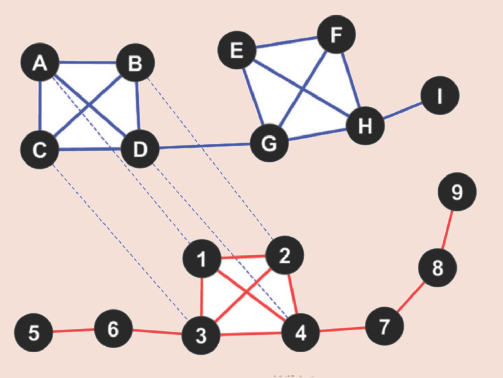
\includegraphics[height=0.25\textheight]{pic/lna.png}
\captionsetup{margin=50pt}
\caption{局部网络匹配,其中[1,2,3,4]可以和[A,B,C,D]匹配,也可以和[E,F,G,H]匹配 \cite{atias2012comparative} \label{fig:lna}}
\end{figure}
而全局匹配,顾名思义,则是从整体上来对一个网络进行匹配,它匹配的不是一个网络的子图,而是整个网络,并且,点与点之间的关系是一对一(one-to-one),而不是像LNA是多对多(many-to-many)。

\begin{figure}[htbp]
\centering
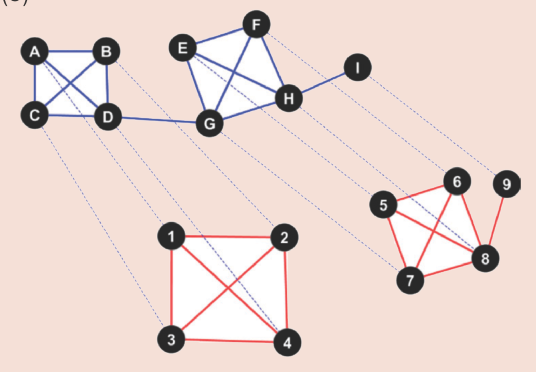
\includegraphics[height=0.25\textheight]{pic/gna.png}
\captionsetup{margin=50pt}
\caption{全局网络匹配,可以看到所有点都得到了匹配 \cite{atias2012comparative} \label{fig:gna}}
\end{figure}
相比于LNA注重两个网络中的局部相似性,GNA更关心一个网络在整体上和另一个网络的相似程度,近来越来越得到学者们的关注。

常见的局部网络匹配算法有PathBLAST\cite{kelley2004pathblast},NetworkBLAST\cite{sharan2005conserved},NetAlign\cite{liang2006netalign},MaWISh\cite{koyuturk2006pairwise}和Graemlin\cite{flannick2006graemlin}。之后,大量的全局网络匹配算法被提出,常见的有IsoRank\cite{singh2008global,liao2009isorankn},GRAAL\cite{kuchaiev2011integrative,malod2015graal,kuchaiev2010topological,milenkovic2010optimal,memivsevic2012c},MAGNA和MAGNA++\cite{saraph2014magna,vijayan2015magna++},SPINAL\cite{aladaug2013spinal},PINALOG\cite{phan2012pinalog},Netcoffee\cite{hu2013netcoffee},BEAMS\cite{alkan2014beams}。而本文研究的重点也是全局网络匹配。

IsoRank\cite{singh2008global}可以说是全局匹配算法中的先驱,它定义了两个网络间任意点对之间的相似度分数(score),这个分数由这个两个点代表的蛋白质的结构信息(structural similarity)和序列信息(protein sequence similarity)同时决定。然后以这个分数为标准,通过一定的策略,得到最终的匹配结果。类似于IsoRank,GRAAL一系列方法也定义了两个点之间的相似程度,不过不同于IsoRank的是,GRAAL一系列算法通过衡量两个点之间的小图度数相似度(graphlet-degree)作为两个点之间的相似度分数。GRAAL\cite{kuchaiev2010topological}是这一系列方法中的第一个方法,它根据计算得到的相似度分数,从高到低选择种子点对(seed pair),然后考虑这个点对的邻居集合(neighbour set)间的相似度,贪心地选择新的匹配点对。H-GRAAL\cite{milenkovic2010optimal}则用了二分图和匈牙利算法来优化GRAAL中的贪心过程,使得产生的匹配结果更好,而代价就是运行时间的增加。而MI-GRAAL\cite{kuchaiev2011integrative}则可以用不同的相似度分数来进行点对匹配。L-GRAAL\cite{malod2015graal}则是GRAAL系列算法中最近提出来的算法,它将图匹配的问题建模成了一个线性规划的问题,然后从该问题中得到一个较优的解。SPINAL算法\cite{aladaug2013spinal}是一种迭代式算法,它通过不断扩展已匹配点周围的邻居点对来生成新的匹配点对。MAGNA\cite{saraph2014magna}则运用了遗传算法来对已有匹配结果进行改进。

到目前为止,既有的网络匹配算法,无论是局部网络匹配算法还是全局网络匹配算法,都是针对静态PPI网络的匹配。也就是说,待匹配的目标网络是单一不变的。然而,生物细胞中的生命活动往往是动态的,而与细胞生命活动息息相关的蛋白质相互作用网络,其实是随时间变化的,可能在前一时刻两者还有相互作用的蛋白质,在后一时刻由于细胞生命活动的变更,而变得没有相互作用了。虽然将生物体蛋白质之间的相互作用以一个静态的PPI网络进行建模,已经能够体现蛋白质之间的相互作用了,但是这种表示方式并不能体现时间维度上的特征。

最近,关于动态PPI网络上(dynamic protein-protein interaction networks)的课题越来越多,预示着学者们对动态PPI网络的重视逐日增加。因此,为了更好地挖倔PPI网络的动态信息,在动态PPI网络上作PPI网络匹配是很有意义的一个新课题。虽然有不少文章的工作是基于动态PPI网络的\cite{lin2010dynamic,chen2014identifying,wang2013construction},但它们构造动态PPI网络的方式也不尽相同,而且研究的问题也不同。故针对本文研究的问题,我们需要一个完整的动态PPI网络概念以及对应的匹配问题的定义。

随之而来的问题就是,针对动态的PPI网络,能否提出切实有效的匹配算法呢?这也是本文要研究的重点内容。

本文首先提出了动态PPI网络的概念,然后定义了动态PPI网络匹配(alignment of dynamic protein-protein interaction networks)这一全新的问题,最后设计了一种算法叫SGOPT(SeGment tree OPTimization),并用完整的,系统的实验证明了该算法的效果。SGOPT是一种基于既有静态PPI网络匹配算法的方法,它是一种迭代式地,不断更新当前解的,基于局部调整策略的算法。它可以和任意既有静态PPI网络匹配算法相结合,产生更优秀的匹配。
%@@@@@@@@@@@@@@@@@@@@@@@@@@@@@@@@@@@@@@@@@@@@@@@@@@@@@@@@@@@
\section{本文结构}

第二章着重介绍了一些本文要研究的问题的相关概念,以及一些相关工作。第三章介绍了本文的主要贡献,包括动态PPI网络概念的定义,问题的定义,SGOPT算法的详细介绍等。第四章是实验分析部分。第五章总结文章。
